\setboolean{IsHalfPage}{false}%
\setboolean{IsHalfPageLeftCol}{false}%
\setboolean{IsHalfPageRightCol}{false}%
\def\ChapterTitle{%
	Container Village
}
\def\ChapterUrl{%
	https://arnottferels.github.io/work/YYYYYYYYYYYYYYYYYYYY
}
\def\ChapterDescription{%
	Redefining Urban Living with Kampong Container
}
\def\ChapterDetailsLine{%
	Professional Work -- 2019 | Urban Housing Research; Modular Design | East Jakarta, Indonesia
}
\def\ChapterDetailsTabular{%
	\begin{tabular}{@{}ll}
		\textbf{Type}          & Professional Competition by Perumnas (National Urban Development Corporation) \\
		\textbf{Award}         & Top~10 \& Semifinalist                                                        \\
		\textbf{Contributions} & Research, Concept, Design, BIM Modeling \& Visualization                      \\
		\textbf{Software}      & Revit, Lumion \& Adobe Photoshop                                              \\
		\textbf{Collaborators} & Cathleen Charity \& Oliver Kenny                                              \\
	\end{tabular}
}
\def\ChapterAbstract{%
	This project revolutionizes urban living in East Jakarta by employing an innovative housing approach using modular containers. Strategically placed near vital amenities, the development introduces two housing types, Type A and Type B, catering to different resident configurations. The inclusion of a plugin system boosts user mobility and facilitates an efficient, organic building process within the Kampong Container. Drawing inspiration from Indonesian culture, communal spaces on each floor cultivate a sense of community, encouraging self-economy and self-energy. Prioritizing sustainability and cultural values, the project addresses Jakarta's housing requirements while reshaping contemporary living standards.
}
\StartTwoColumnLayout
\chapter*{\ChapterTitle}\addcontentsline{toc}{chapter}{\ChapterTitle}
\ChapterSetTocAddData{\ChapterDetailsLine}
\ChapterSetDetailsData{\ChapterDescription}{\ChapterDetailsLine}{\ChapterDetailsTabular}
\RuleAbstract
\ChapterAbstract
\vspace{\baselineskip}%
\par%
\edef\MinipageHeight{\the\dimexpr(\pagegoal-\pagetotal-\textheight-\baselineskip)\relax}
\begin{minipage}[t][\MinipageHeight][t]{\linewidth}
	\section*{
	  Introduction
	 }
	An innovative housing project in East Jakarta repurposes a vacant plot initially designated for high-rises. Strategically located near TransJakarta bus stops, mosques, and schools, the site leverages Jakarta's container accessibility. Challenges include ergonomic adjustments and affordable housing demand. Opportunities involve surplus containers, Gen Y and Z entering the market, and addressing wealth gaps. The project aims to meet Jakarta's housing needs by capitalizing on container advantages and embracing the city's unique characteristics.
	\vfill
	\section*{
	  Method: Unit Configuration
	 }
	%
\begin{figure}[H]
	\centering
	\includesvg[width=\linewidth]{src/graphics/container-village--method-unit-configuration.svg}
	\label{
		fig:container-village--method-unit-configuration
	}
\end{figure}

	\vfill
	%
\begin{figure}[H]
	\centering
	
\includegraphics[width=\linewidth]{src/graphics/container-village--physical-model.jpg}
	\caption*{%
		Architectural model illustrating the operational principles of the plugin system.
	}%
	\label{%
		fig:container-village--physical-model
	}%
	\vspace{0pt}%
\end{figure}%

\end{minipage}
\columnbreak%
\begin{minipage}[t][\textheight][t]{\linewidth}
	\section*{
	  Development Phase
	 }
	\vspace{-0.25cm}%
	\begin{figure}[H]
	\centering
	\includesvg[width=\linewidth]{src/graphics/container-village--development-phase.svg}
	\label{
		fig:container-village--development-phase
	}
\end{figure}

	\vfill
	\section*{
	  Plugin System
	 }
	\vspace{-0.25cm}%
	\begin{center}
		\begin{minipage}[t]{0.8\linewidth}
			%
\begin{figure}[H]
	\centering
	\includesvg[width=\linewidth]{src/graphics/container-village--plugin-system.svg}
	\label{
		fig:container-village--plugin-system
	}
\end{figure}

		\end{minipage}
	\end{center}
	\vspace{-\baselineskip}
	\vfill
	\vspace{-\baselineskip}
	\section*{
	  Design
	 }
	\vspace{-0.25cm}%
	\setlength{\MinipageGap}{0.5cm}
	\setlength{\MinipageAWidth}{\dimexpr ((0.5875\linewidth) - (\MinipageGap))\relax}%
	\setlength{\MinipageBWidth}{\dimexpr (\linewidth - \MinipageAWidth - \MinipageGap)\relax}
	\begin{minipage}[t]{\MinipageAWidth}%
		%
\begin{figure}[H]
	\centering
	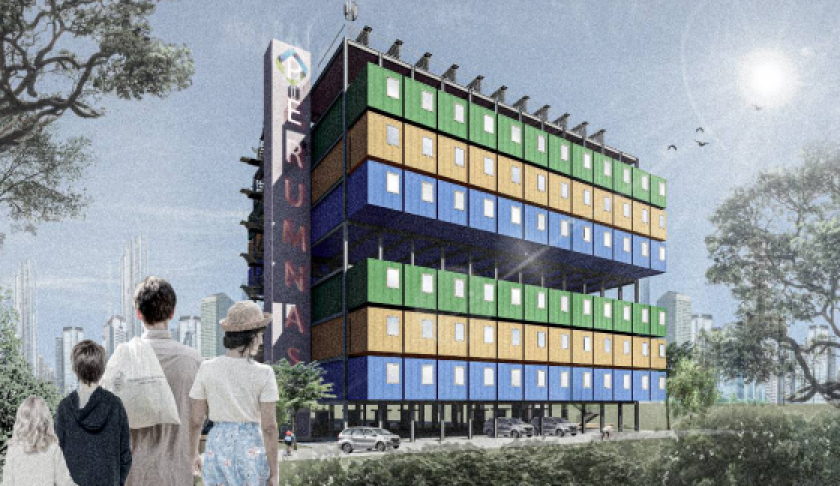
\includegraphics[width=\linewidth]{src/graphics/container-village--perspective-01.jpg}
	\label{
		fig:container-village--perspective-01
	}
\end{figure}

	\end{minipage}%
	\hspace{\MinipageGap}%
	\begin{minipage}[t]{\MinipageBWidth}%
		%
\begin{figure}[H]
	\centering
	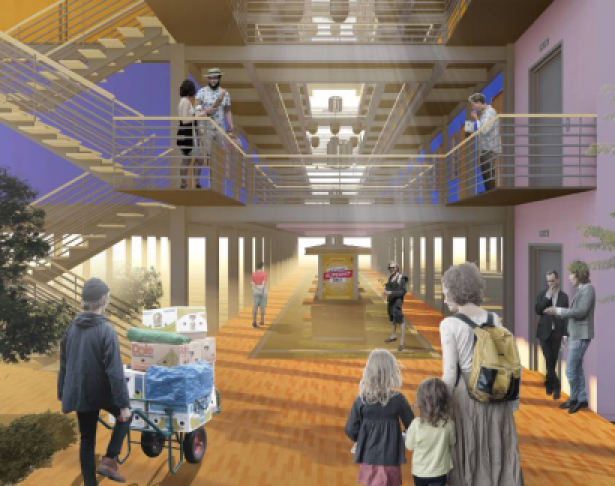
\includegraphics[width=\linewidth]{src/graphics/container-village--perspective-02.jpg}
	\label{
		fig:container-village--perspective-02
	}
\end{figure}

	\end{minipage}%
	\vfill
\end{minipage}
\newpage
\setlength{\columnsep}{0.25cm}%
\begin{multicols}{2}
	%
\begin{figure}[H]
	\centering
	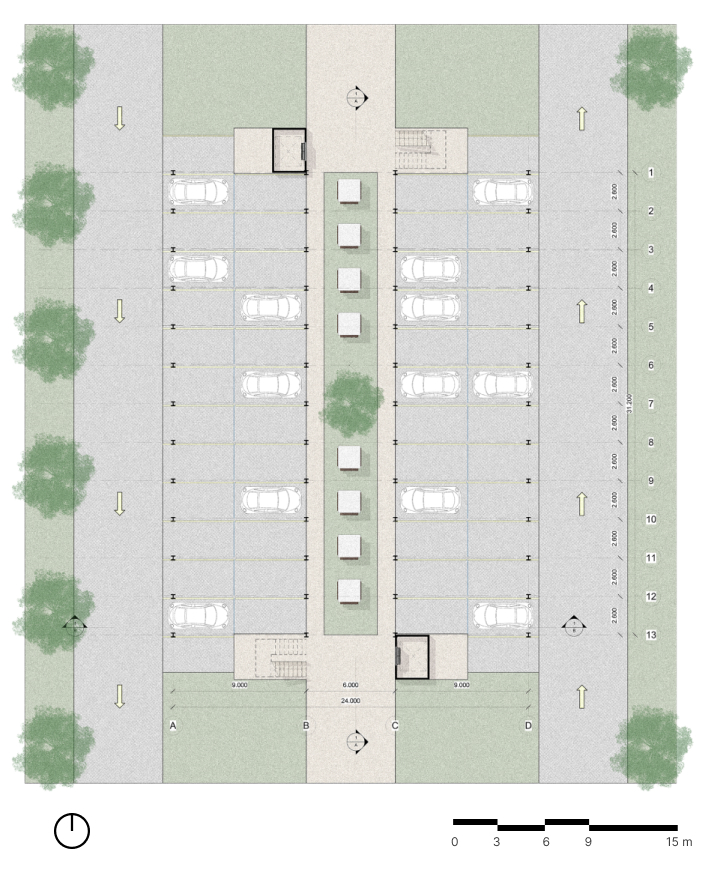
\includegraphics[width=\linewidth]{src/graphics/container-village--level-01.jpg}
	\caption*{%
		Level~1 (GF)
	}
	\label{
		fig:container-village--level-01
	}
\end{figure}

	%
\begin{figure}[H]
	\centering
	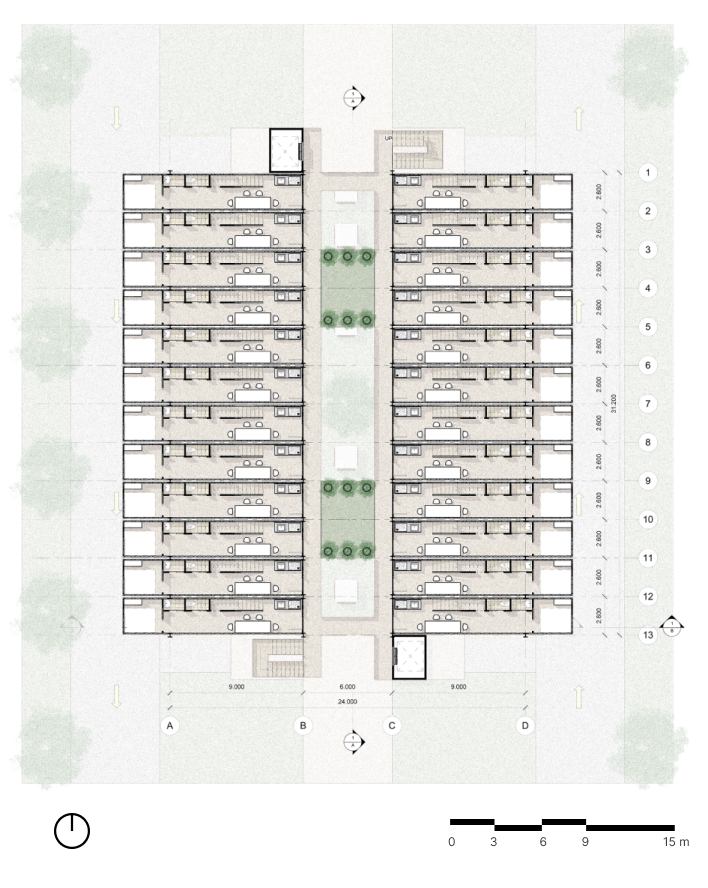
\includegraphics[width=\linewidth]{src/graphics/container-village--level-02.jpg}
	\caption*{%
		Level~2 (Type B)
	}
	\label{
		fig:container-village--level-02
	}
\end{figure}

\end{multicols}
\section*{
  Concept: Self-economy
 }
%
\begin{figure}[H]
	\centering
	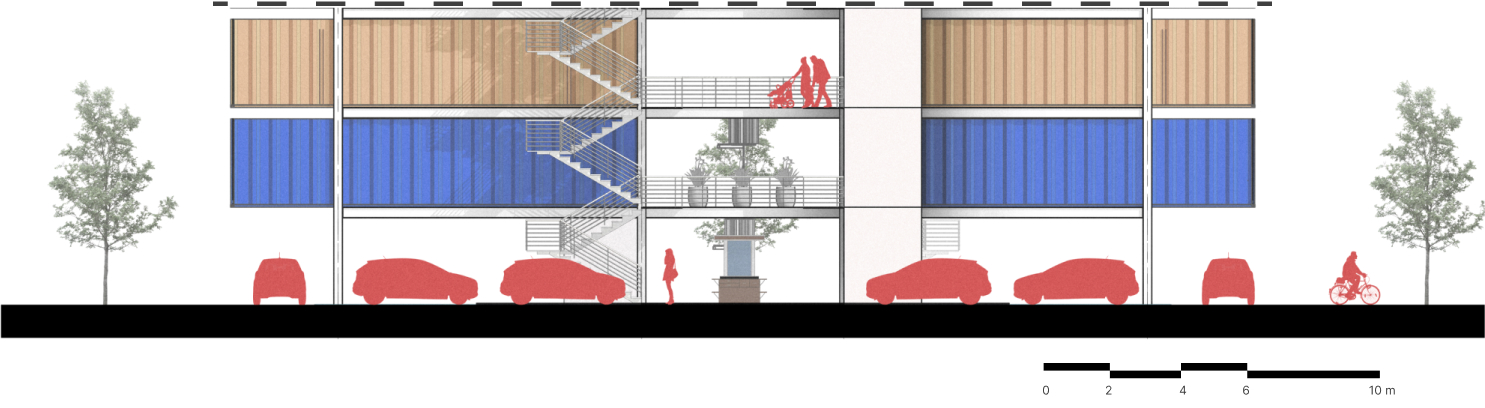
\includegraphics[width=\linewidth]{src/graphics/container-village--concept-self-economy.jpg}
	\label{
		fig:container-village--concept-self-economy
	}
\end{figure}

The communal spaces on each floor deck and atrium, inspired by Indonesian culture, encourage a sense of togetherness and gathering. The Indonesian cultural characteristics of the market concept in the Kampong Container (Container Village) can also contribute to the local economy.
\vfill
\begin{minipage}{\linewidth}
	\setlength{\MinipageGap}{0.5cm}
	\setlength{\MinipageAWidth}{\dimexpr ((0.55\linewidth) - (\MinipageGap))\relax}%
	\setlength{\MinipageBWidth}{\dimexpr (\linewidth - \MinipageAWidth - \MinipageGap)\relax}
	\begin{minipage}[t]{\MinipageAWidth}%
		%
\begin{figure}[H]
	\centering
	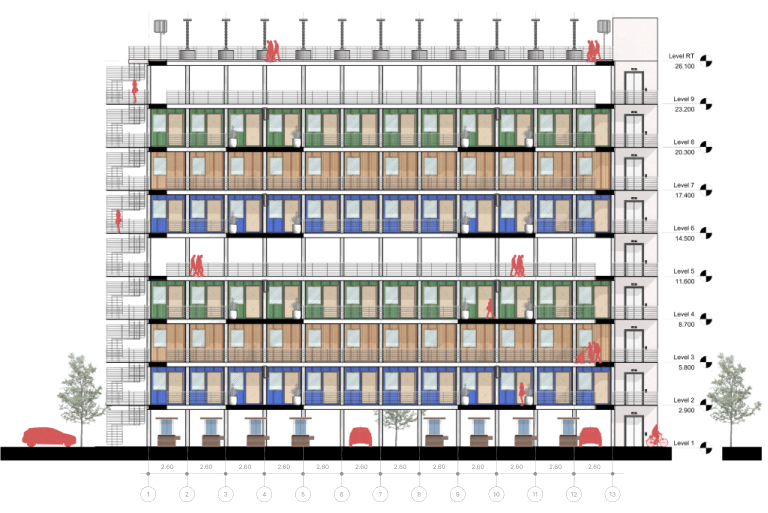
\includegraphics[width=\linewidth]{src/graphics/container-village--section-aa.jpg}
	\caption*{%
		Section A-A
	}
	\label{
		fig:container-village--section-aa
	}
\end{figure}

	\end{minipage}%
	\hspace{\MinipageGap}%
	\begin{minipage}[t]{\MinipageBWidth}%
		%
\begin{figure}[H]
	\centering
	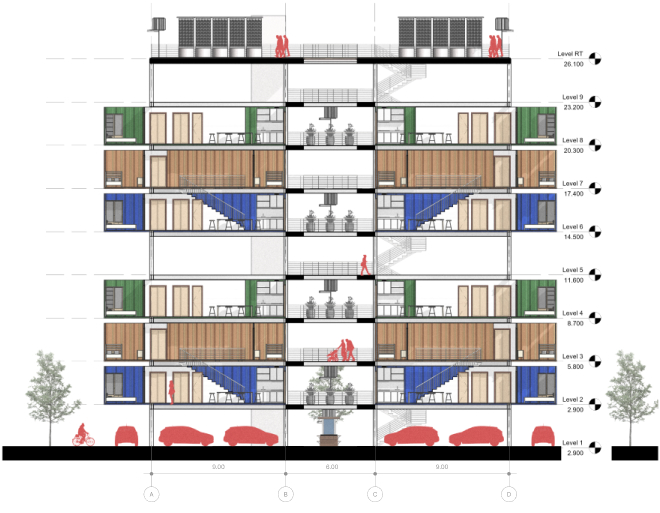
\includegraphics[width=\linewidth]{src/graphics/container-village--section-bb.jpg}
	\caption*{%
		Section B-B
	}
	\label{
		fig:container-village--section-bb
	}
\end{figure}

	\end{minipage}%
\end{minipage}
\columnbreak%
\setlength{\columnsep}{0.25cm}%
\begin{multicols}{2}
	%
\begin{figure}[H]
	\centering
	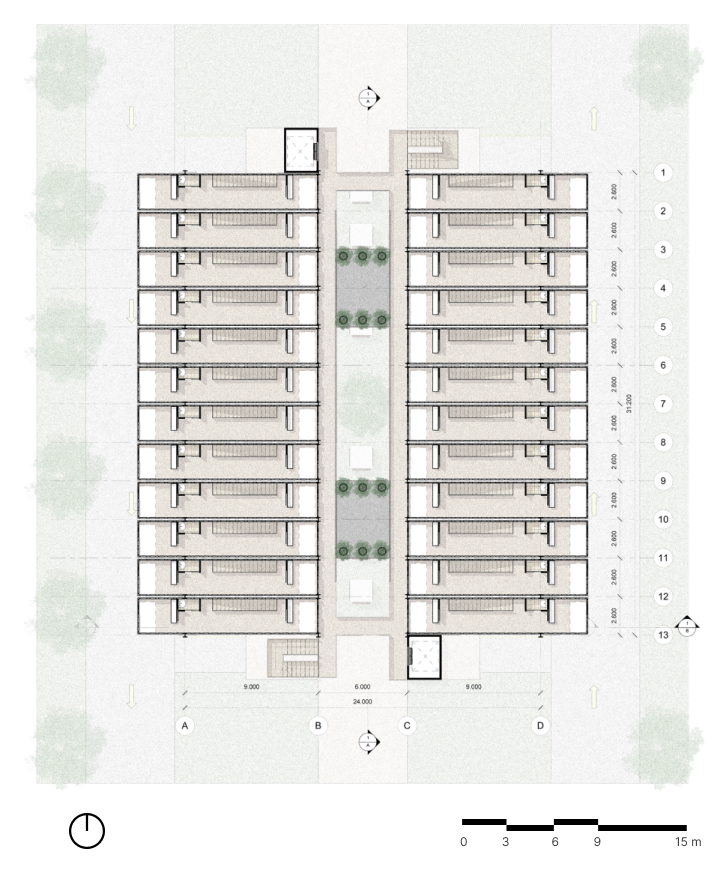
\includegraphics[width=\linewidth]{src/graphics/container-village--level-03.jpg}
	\caption*{%
		Level~3 (Type B)
	}
	\label{
		fig:container-village--level-03
	}
\end{figure}

	%
\begin{figure}[H]
	\centering
	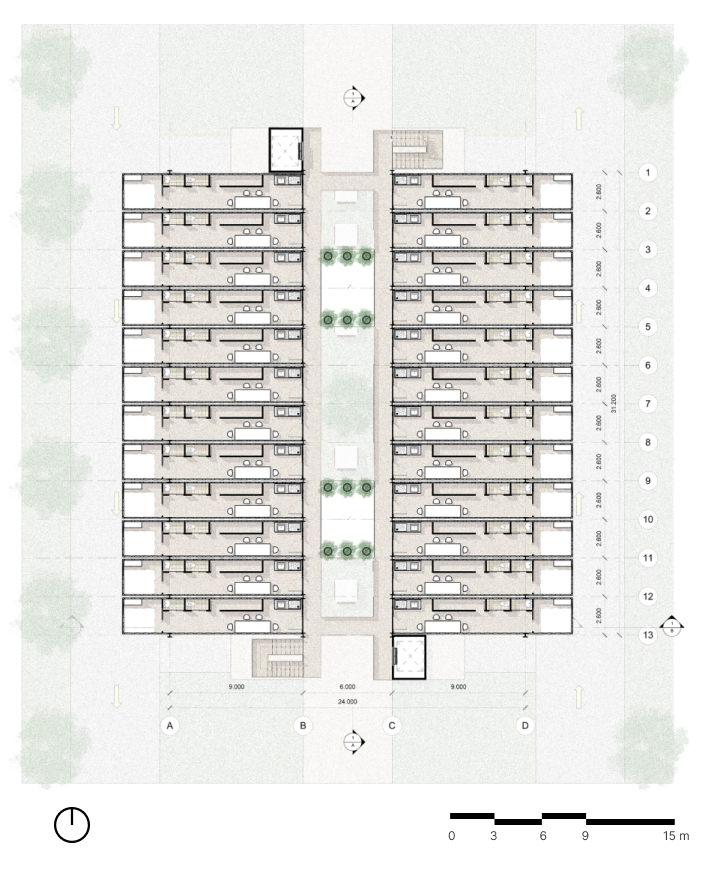
\includegraphics[width=\linewidth]{src/graphics/container-village--level-04.jpg}
	\caption*{%
		Level~4 (Type B)
	}
	\label{
		fig:container-village--level-04
	}
\end{figure}

\end{multicols}
\setlength{\columnsep}{0.25cm}%
\begin{multicols}{2}
	\section*{
	  Concept: Self-energy
	 }
	%
\begin{figure}[H]
	\centering
	\includesvg[width=\linewidth]{src/graphics/container-village--concept-self-energy.svg}
	\label{
		fig:container-village--concept-self-energy
	}
\end{figure}

	\vspace{-\baselineskip}%
	The rooftop and decks of each floor are equipped with ecological independent energy sources such as vertical gardens, solar panels, fish ponds, and wind turbines.
	\columnbreak%
	\section*{
	  Concept: Self-installation
	 }
	%
\begin{figure}[H]
	\centering
	\includesvg[width=\linewidth]{src/graphics/container-village--concept-self-installation.svg}
	\label{
		fig:container-village--concept-self-installation
	}
\end{figure}

	\vspace{-\baselineskip}%
	The plugin system, which allows for user mobility, contributes to the high efficiency and organic building process in the Kampung Kontainer (Container Village).
\end{multicols}
\EndTwoColumnLayout
